\documentclass[serif,9pt,xcolor=dvipsnames]{beamer}
\usetheme{default}

%\usepackage[english]{babel}    % deutsche Sonderzeichen, Trennmuster, etc
\usepackage[german]{babel}    % deutsche Sonderzeichen, Trennmuster, etc

\usepackage[T1]{fontenc} 
\usepackage[utf8]{inputenc}  % deutsche Umlaute


\usetheme[]{Warsaw}
%\usetheme[]{Rochester}

%  \usecolortheme[named=Brown]{structure} 
%\usecolortheme[]{crane} 
%\usecolortheme[]{rose} 
\usecolortheme[]{christian1} 

% Mathekram
%\usepackage{amsmath}
%\usepackage{amsfonts}
%\usepackage{amssymb}

% Graphiken
%\usepackage{epsfig}            % Paket zum Einbinden von postscript Graphiken
\usepackage{graphicx}		% Andere Graphikdateien einbinden
\usepackage{float}             % Hilfesmakros beim Positionieren von Graphiken
\usepackage{color}
%\usepackage{subfig}
\usepackage{textcomp}

\usepackage[sc]{mathpazo}	%FONT

\usepackage{relsize} % Notwenfig für verbatim
\usepackage{listings}
\usepackage{verbatim}


%% GLEGRAPHICS
\graphicspath{{./bilder/gleplots/}}

\newcommand{\includeglegraphics}[1]{  
%\includegraphics[]{#1.pdf}
\input{#1.inc}   
}

% \newcommand{\listing}[1]{
%    {\small 
%   \begin{lstlisting}
%    
%   \end{lstlisting}}
% }

\newcommand{\Th}{\vartheta}

%\newcommand{\Th}{\vartheta}


\definecolor{feedforwardpath}{rgb}{0.0,1,0.0}
\definecolor{feedbackpath}{rgb}{1.0,0.0,0.0}

\DeclareRobustCommand{\vec}[1]{{\mbox{\mathversion{bold}\ensuremath{#1}}}}
\DeclareRobustCommand{\mat}[1]{{\mbox{\mathversion{bold}\ensuremath{#1}}}}

\title[]{ORTD --- The Open Realtime Dynamics Toolbox}
	\subtitle{} %Mehrgrößenregelung einer Neuro-Prothese zur Generierung von Bewegungen  der oberen Extremität mittels Neuromuskulärer Elektrostimulation (NMES)
\date{2011}
\author{Christian Klauer$^{1}$\\
{\tiny $^{1}$Fachgebiet Regelungssysteme, Technische Universität Berlin\\
Kontakt: klauer@control.tu-berlin.de}
}




\begin{document}
% \frame[plain]{\titlepage}

\author{Christian Klauer$^{1}$}



\begin{frame}
  \maketitle
\end{frame}


\begin{frame}

OpenRTDynamics is

 \begin{itemize}
  \item A simulator for time-discrete dynamical systems
  \item A set of Scilab functions for describing such dynamical systems via a block / signal based description.
  \item Additional things like
  \begin{itemize}
    \item A remote control interface
   \end{itemize}
 \end{itemize}

Compared to other simulation environments it features:
\begin{itemize}
 \item Nested-schematics: The possibility to include multiple schematics within top level schematics. Online switching between the sub-simulations is possible.
 \item A new way of defining schematics, which enables well structured code, which is easy to maintain as projects get bigger.
\item Does not require a code compilation step for generating real-time code, because online interpretation is used for execution.
\end{itemize}


\end{frame}



\begin{frame}

 \frametitle{General Overview}



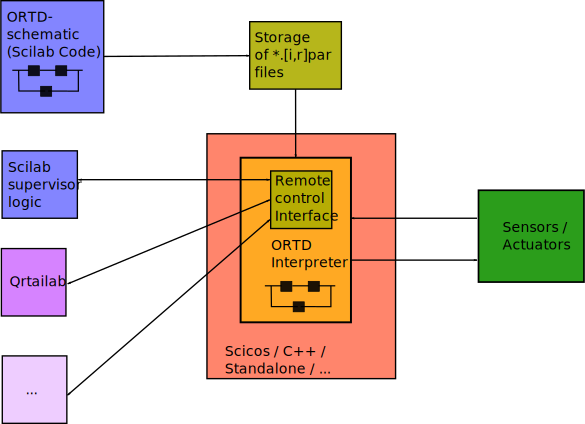
\includegraphics[trim=0mm 0mm 0mm 0mm, clip,width=0.95\linewidth]{../pictures/ortd_principle.pdf}

\end{frame}



% \begin{frame}
% \frametitle{Signals and Blocks in ORTD}
% 
% \begin{itemize}
%  \item A special Scilab variable type is introduced, which represents a signal.
% \item Blocks are represented by calls to special Scilab functions, which have input and output signals.
% \end{itemize}
% 
% \end{frame}
% 



\begin{frame}[fragile]
  \frametitle{Signals and Blocks in ORTD}

\begin{itemize}
 \item A special Scilab variable type is introduced, which represents a signal.
 \item Blocks are represented by calls to special Scilab functions, which have input and output signals.
\end{itemize}

\begin{itemize}
 \item A linear combination of two signals ( $y=u_1 - u_2$ ) would look like:
\end{itemize}


{\small 
\begin{lstlisting}
   [sim, y] = ld_add(sim, defaultevents, list(u1, u2), [ 1, -1 ] );
\end{lstlisting}}
  

\begin{itemize}
 \item A time-discrete transfer function is implemented like this:
\end{itemize}

{\small 
\begin{lstlisting} 
    [sim, y] = ld_ztf(sim, defaultevents, u, (1-0.2)/(z-0.2) );
\end{lstlisting}}


\begin{itemize}
 \item Looks very similar to normal Scilab-Code, but for all calculations the toolbox functions have to be used.
\end{itemize}
 


\end{frame}



\begin{frame}[fragile]
\frametitle{Signals and Blocks in ORTD}
 
 
{\small 
\begin{lstlisting}
   [sim, y] = ld_add(sim, defaultevents, list(u1, u2), [ 1, -1 ] );
\end{lstlisting}}
 
 \begin{itemize}
  \item The variable \texttt{sim} is used to emulate Object-Orientated behaviour in Scilab.
\item \texttt{defaultevents} defines a set of events that will be forwarded to the block.
 \end{itemize}

 
\end{frame}



\begin{frame}[fragile]
  \frametitle{A working example -- part 1}

\begin{itemize}
 \item Every schematic is defined within a Scilab function.
\end{itemize}


{\small 
\begin{lstlisting} 
// This is the main top level schematic
function [sim, outlist] = schematic_fn(sim, inlist)
   u1 = inlist(1); // Simulation input #1
   u2 = inlist(2); // Simulation input #2
   
  // sum up two inputs
  [sim,out] = ld_add(sim, defaultevents, list(u1, u2), [1, 1] );
  
  // save result to file
  [sim, save0] = ld_dumptoiofile(sim, defaultevents, ...
       "result.dat", out);
  
  // output of schematic
  outlist = list(out); // Simulation output #1
endfunction
\end{lstlisting}}

\begin{itemize}
 \item It takes the simulation object \texttt{sim} as well as a list of in- and  outputs.
\end{itemize}


\end{frame}


\begin{frame}[fragile]
  \frametitle{A working example -- part 2}

\begin{itemize}
 \item A schematic is generated via the following code. 
 \item The function \texttt{libdyn\_setup\_schematic} calls the function describing the schematic.
\end{itemize}


{\small 
\begin{lstlisting} 
defaultevents = [0]; // main event

// set-up schematic by calling the user defined
// function "schematic_fn"
insizes = [1,1]; outsizes=[1];
[sim_container_irpar, sim]=libdyn_setup_schematic(schematic_fn, ...
                            insizes, outsizes);

// Initialise a new parameter set
parlist = new_irparam_set();

// pack simulations into irpar container with id = 901
parlist = new_irparam_container(parlist, sim_container_irpar, 901);

// irparam set is complete convert to vectors
par = combine_irparam(parlist);

// save vectors to a file
save_irparam(par, 'simple_demo.ipar', 'simple_demo.rpar');
\end{lstlisting}}

\end{frame}


\begin{frame}[fragile]
  \frametitle{A working example -- part 3}
 \begin{itemize}
  \item This Scilab-Script will generate two files \texttt{simple\_demo.ipar} and \texttt{simple\_demo.rpar}, which contain a encoded definition of the whole schematic.
\item These file are then loaded by the provided interpreter library and executed.
\item The interpreter can be interfaced via
  \begin{itemize}
   \item the executable \texttt{libdyn\_generic\_exec}
   \item the provided Scicos-Block
   \item third party C++ Code
  \end{itemize}
 \end{itemize}

\end{frame}


\begin{frame}[fragile]
 \frametitle{Superblocks: definition}
 
\begin{itemize}
 \item Superblocks are introduced by writing a new Scilab function.
\end{itemize}

{\small 
\begin{lstlisting} 
function [sim, y] = ld_mute( sim, ev, u, cntrl, mutewhengreaterzero )
    [sim, zero] = ld_const(sim, ev, 0);
    
    if (mutewhengreaterzero == %T) then
      [sim,y] = ld_switch2to1(sim, ev, cntrl, zero, u);
    else
      [sim,y] = ld_switch2to1(sim, ev, cntrl, u, zero);
    end
endfunction
\end{lstlisting}}

\begin{itemize}
 \item The example describes a superblock, which has two inputs \texttt{u} and \texttt{cntrl} and one output \texttt{y}.
\item \texttt{mutewhengreaterzero} describes an parameter.
\item \textbf{NOTE}: With the if / else construction a superblock can have different behaviour depending on a parameter! (This enables great possibilities for creating reusable code)
\end{itemize}


\end{frame}


\begin{frame}[fragile]
 \frametitle{Superblocks: Usage}
 
 \begin{itemize}
  \item Once defined, the superblock can be used like any other ORTD-Block:
 \end{itemize}

 
 {\small 
\begin{lstlisting} 
 [sim, y] = ld_mute( sim, ev, u=input, cntrl=csig, ...
                     mutewhengreaterzero=%T ) 
\end{lstlisting}}

\end{frame}




\begin{frame}[fragile]
 \frametitle{Feedback Loops}

  \begin{itemize}
   \item To create a signal, which comes from an (for now) unknown source \texttt{libdyn\_new\_feedback} is used:
  \end{itemize}


  {\small 
  \begin{lstlisting} 
  [sim, feedback] = libdyn_new_feedback(sim);
  \end{lstlisting}}

  \begin{itemize}
   \item Now, the signal \texttt{feedback} can be used like an usual signal.
   \item At some point in the ongoing code the loop is closed via \texttt{libdyn\_close\_loop}, which means \texttt{feedback} is assigned to a real signal \texttt{y}:
  \end{itemize}

  {\small 
  \begin{lstlisting} 
  [sim] = libdyn_close_loop(sim, y, feedback);
  \end{lstlisting}}
  
\end{frame}





\begin{frame}[fragile]
 \frametitle{Feedback Loops: An example}


  {\small 
  \begin{lstlisting} 
function [sim, y] = limited_int(sim, ev, u, min__, max__, Ta)
  // Implements a time discrete integrator with saturation
  // of the output between min__ and max__
  // 
  // u * - input
  // y * - output
  // 
  // y(k+1) = sat( y(k) + Ta*u , min__, max__ )

    [sim, u__] = ld_gain(sim, ev, u, Ta);
    
    // create z_fb, because it is not available by now
    [sim,z_fb] = libdyn_new_feedback(sim);
    
    // do something with z_fb
    [sim, sum_] = ld_sum(sim, ev, list(u__, z_fb), 1, 1);
    [sim, tmp] = ld_ztf(sim, ev, sum_, 1/z);

    // Now y becomes available
    [sim, y] = ld_sat(sim, ev, tmp, min__, max__); 

    // assign z_fb = y    
    [sim] = libdyn_close_loop(sim, y, z_fb);    
endfunction
\end{lstlisting}}


\end{frame}








\begin{frame}

\begin{itemize}
 \item More advanced features like mathematical formula parsing, vectors, nesting schematics and the remote control interface are following. For now have a look at the website: \texttt{openrtdynamics.sf.net}.
  \item Additionally, have a look at the demonstrations within the \texttt{examples/} directory of the toolbox. They also run the interpreter once you execute the Scilab script, so you immediately get an result.
\end{itemize}

\end{frame}



\end{document}
